\begin{frame}
\section{Konzept}
\frametitle{Was ist Apache Kafka?}
\begin{columns}[T]
	\begin{column}[T]{0.49\textwidth}
		
	\end{column}
	\begin{column}[T]{0.49\textwidth}
		
\end{column}
\end{columns}

\centering
\begin{figure}[h]
	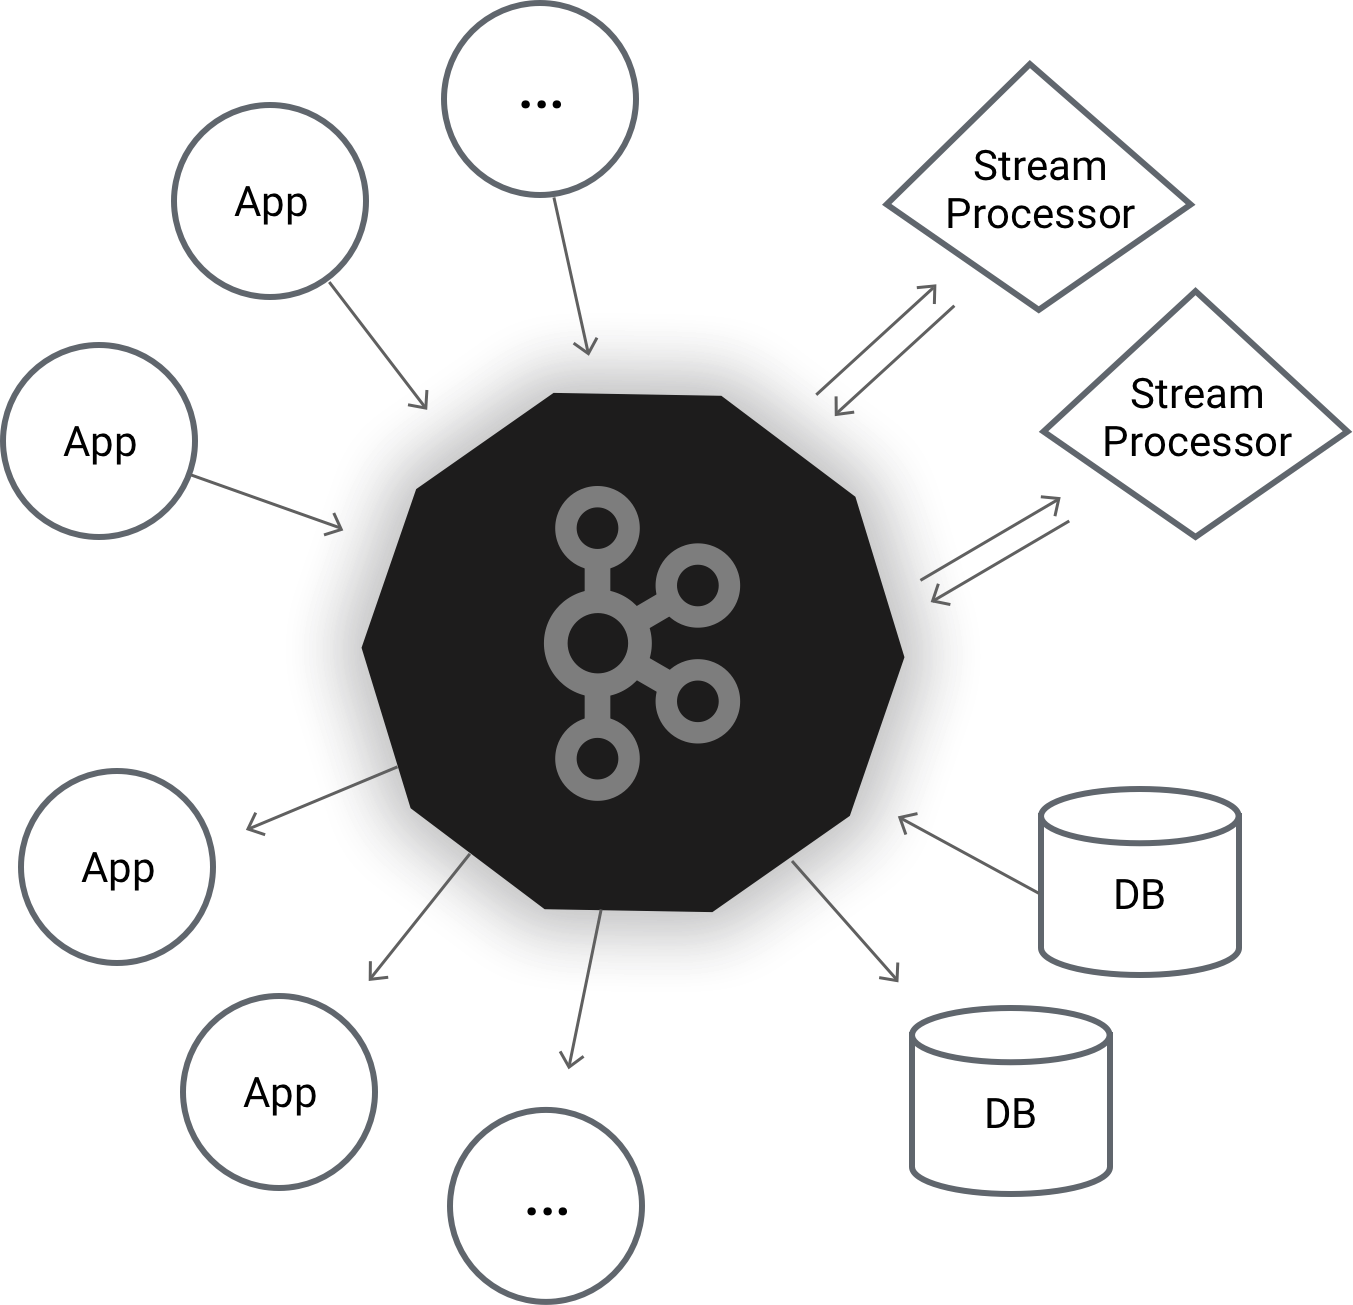
\includegraphics[scale=0.1]{figure/kafka_diagram.png}
\end{figure}

Apache Kafka ist eine verteilte skalierbare Streaming Plattform.
\end{frame}


\begin{frame}
\frametitle{Eigenschaften}
Kafka ...
\begin{itemize}
	\item ist ein Message Queuing System
	\item kann Nachrichten speichern
	\item kann Nachrichten verarbeiten
	\item kann all das in Echtzeit
\end{itemize}
\end{frame}

\begin{frame}
\frametitle{Unternehmen und Use Cases}

\begin{tabular}{cl}
	\raisebox{-.25\height}{
\includegraphics[scale=0.2]{figure/linkedin_logo.pdf}} 
		& Operational Metrics\\~\\
	\raisebox{-.25\height}{
\includegraphics[scale=0.2]{figure/cisco_logo.pdf}} 
		& OpenSOC (Security Operations Center)\\~\\
	\raisebox{-.25\height}{
\includegraphics[scale=0.08]{figure/netflix_logo.pdf}} 
		& Real-time monitoring and event-processing pipeline\\~\\
	\raisebox{-.25\height}{
\includegraphics[scale=0.2]{figure/spotify_logo.pdf}} 
		& Log Delivery System\\~\\
	\raisebox{-.25\height}{
\includegraphics[scale=0.1]{figure/twitter_logo.pdf}} 
		& Part of Storm stream processing infrastructure
\end{tabular}

\end{frame}

\begin{frame}
\frametitle{Komponenten}
	\centering
	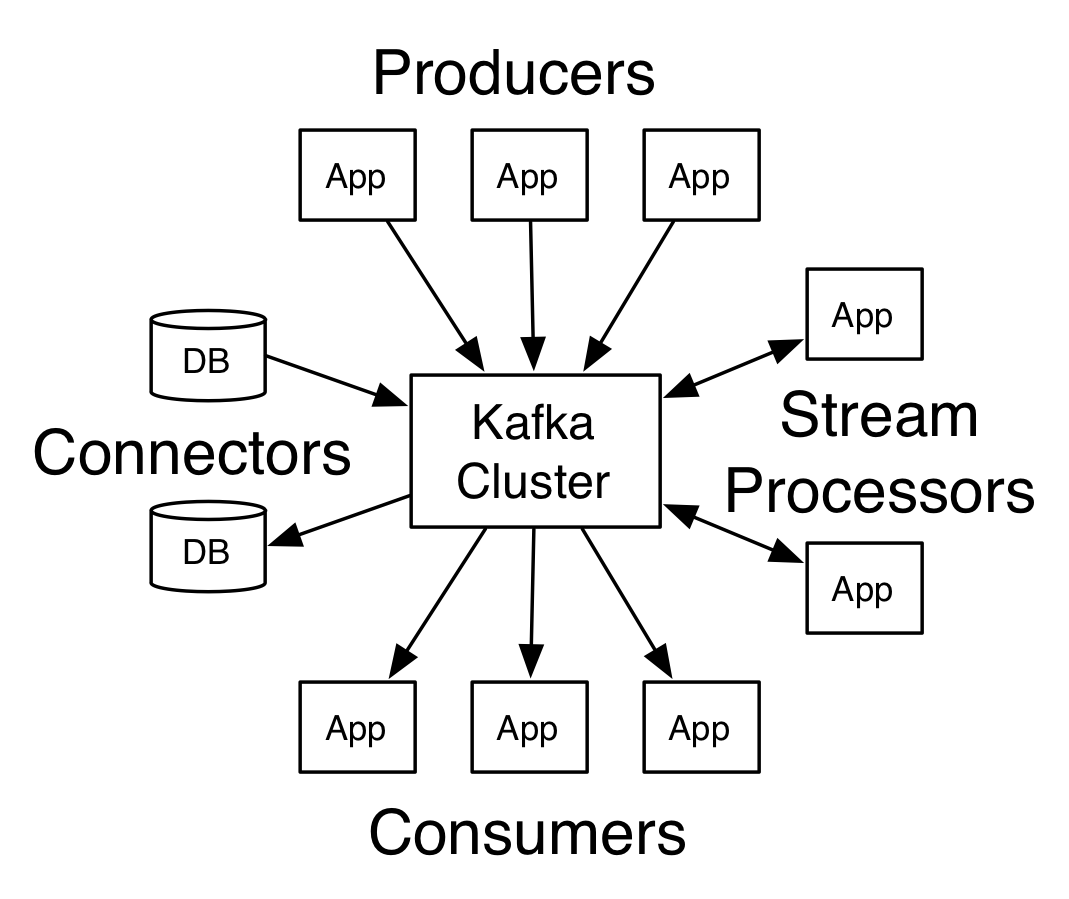
\includegraphics[scale=1.5]{figure/kafka-apis.png}
\end{frame}

\begin{frame}
\frametitle{Queue}
\begin{center}
	\centering
	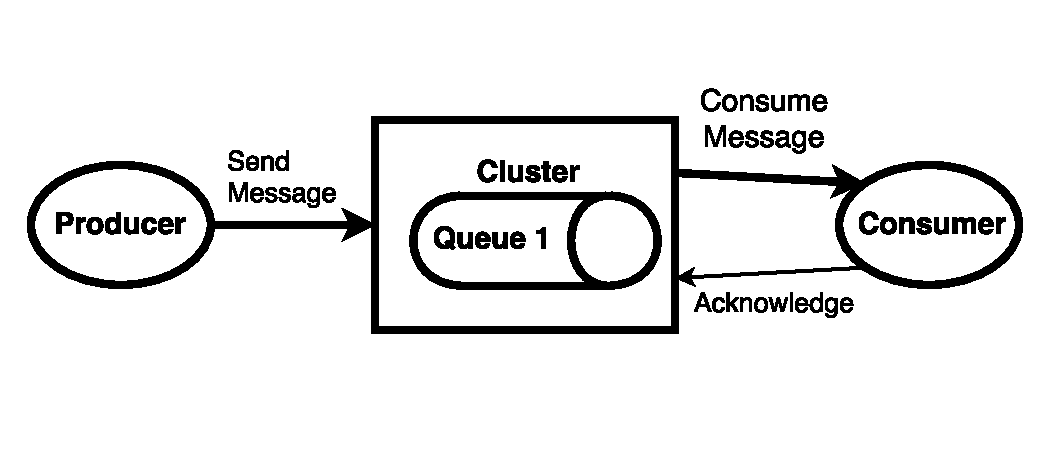
\includegraphics[scale=0.6]{figure/queue_draw.pdf}
\end{center}
\end{frame}

\begin{frame}
\frametitle{Topic}
	\centering
	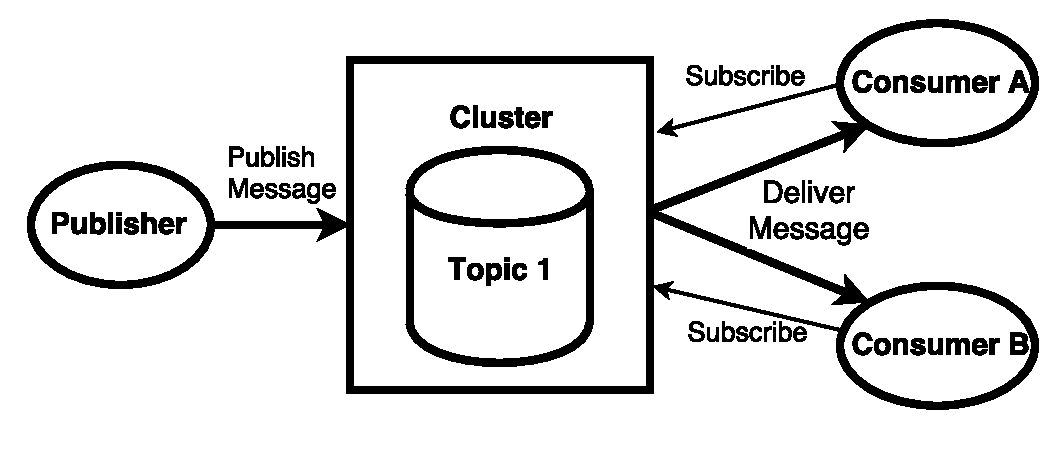
\includegraphics[scale=0.6]{figure/topic_draw.pdf}
\end{frame}

\begin{frame}
\frametitle{Kafka Topics}
\begin{itemize}
	\item Multi-Subscribe ($0$ bis $n$ Consumer)		% Consumergroups - n Anzahl der Partitionen
	\item Kein Push-System
	\item Records in Topics werden persistent gehalten
	\item Topics benötigen eine Cleanup-Policy
		\begin{itemize}
			\item Retention-Time
			\item Retention-Size
			\item Log-Compaction
		\end{itemize}
	\item Topics besitzen Partitionen (partition log)
	\item Guarantees (dazu später mehr)
\end{itemize}
\end{frame}

\begin{frame}
\frametitle{Partitionen}

\end{frame}

\begin{frame}
\frametitle{Kafka Cluster}

\end{frame}



%% Messaging System
\begin{frame}
\frametitle{Kafka als Nachrichtensystem}

Bisher: 
\begin{itemize}
	\item Queueing
	\begin{itemize}
		\item Nachrichten an einen
		\item Nachrichtenverarbeitung skaliert
		\item Nachricht abgerufen = Nachricht weg
	\end{itemize}
	\item Publish-Subscribe
	\begin{itemize}
		\item Nachrichten an alle
		\item Skaliert nicht  			%Jeder bekommt die Nachricht. Daher nicht horizontal skallierbar.
	\end{itemize}
\end{itemize}

\end{frame}

%% Messaging System
\begin{frame}
\frametitle{Kafka als Nachrichtensystem}

\begin{itemize}
	\item Consumer Groups
	\begin{itemize}
		\item Kombiniert Queueing und Publish-Subscribe
		\item Nachrichtenverarbeitung in Gruppen
		\item Mehrere Consumer in einer Gruppe
	\end{itemize}
	\item Vorteile
	\begin{itemize}
		\item Nachrichtenverarbeitung skaliert % Durch Skalierung horizontal Groups und vertical mehrere consumer pro group
	\end{itemize}
	\item Reihenfolge wird eingehalten 
\end{itemize}

\end{frame}

\begin{frame}
\frametitle{Parallelität}

\begin{itemize}
	\item Ordnung 
	\begin{itemize}
		\item Gesichert für alle Consumer Groups
	\end{itemize}
	\item Lastverteilung
		\begin{itemize}
		\item Nachricht 1x pro Consumer Group verarbeitet
	\end{itemize}
\end{itemize}

\end{frame}

%% Storage System
\begin{frame}
\frametitle{Kafka als Datenbank}

\begin{itemize}
	\item Durch Funktionalität bedingt
	\begin{itemize}
		\item Entkopplung sorgt für Speicherbedarf
	\end{itemize}
	\item Daten werden repliziert
	\begin{itemize}
		\item Bestätigungsmechanismen sind vorhanden
		\item Wird erst bestätigt, wenn Replication abgeschlossen ist
	\end{itemize}
\end{itemize}

\end{frame}

\begin{frame}
\frametitle{Kafka als Datenbank - 2}

\begin{itemize}
	\item Performanz bei steigender Datenmenge gleich
	\item Eigenschaften:
	\begin{itemize}
		\item Hohe Performanz
		\item Geringe Latenz %% Für Commit Log Storage
		\item Replikation
		\item Weiterleitung %% Von Nachrichten
	\end{itemize}
\end{itemize}

\end{frame}

\begin{frame}
\frametitle{Kafka für Streams}

\begin{itemize}
	\item Echtzeit Stream-Verarbeitung
	\item Ein Stream Processor:
	\begin{itemize}
		\item Nimmt kontinuierlich Daten aus einem Topic   % Shipments
		\item Bearbeitet die Daten % Preisanpassungen berechnen
		\item Schreibt kontinuierlich Daten in ein Topic % Preisänderungen veröffentlichen
	\end{itemize}
\end{itemize}

\end{frame}


\begin{frame}
\frametitle{Kafka für Streams - 2}

\begin{itemize}
	\item Extra Stream-API wird angeboten
	\begin{itemize}
		\item Ermöglicht komplexere Operationen  % Shipments
		\item Bearbeitet die Daten % Preisanpassungen berechnen
		\item Schreibt kontinuierlich Daten in ein Topic % Preisänderungen veröffentlichen
	\end{itemize}
	\item Kann auch umgehen mit:
	\begin{itemize}
		\item Daten die nicht in Reihenfolge sind  % Shipments
		\item Daten neu verarbeiten wenn sich die Operation ändert % Preisanpassungen berechnen
		\item Status behaftete Operationen sind möglich % Preisänderungen veröffentlichen
	\end{itemize}
\end{itemize}

%The streams API builds on the core primitives Kafka provides: it uses the producer and consumer APIs for input, uses Kafka for stateful storage, and uses the same group mechanism for fault tolerance among the stream processor instances.

\end{frame}

\begin{frame}
\frametitle{Zusammenfassung}

\begin{itemize}
	\item Echtzeit Stream-Verarbeitung
	\item Ein Stream Processor:
	\begin{itemize}
		\item Nimmt kontinuierlich Daten aus einem Topic   % Shipments
		\item Bearbeitet die Daten % Preisanpassungen berechnen
		\item Schreibt kontinuierlich Daten in ein Topic % Preisänderungen veröffentlichen
	\end{itemize}
\end{itemize}

\end{frame}

